%%=============================================================================
%% Onderzoek
%%=============================================================================

\chapter{\IfLanguageName{dutch}{Onderzoek}{Study}}
\label{ch:onderzoek}



In this study a comparison is made between the GNFS algorithm on a classical computer and Shor's algorithm on a quantum computer.
Section \ref{sec:Fields of use} will discuss some other algorithms that can show real benefits of quantum computing in the industry.
\section{The comparison}

To compare both algorithms a list of numbers will be used that both should factor. Each number will be factored 3 times and the time needed will be captured. Then the average of the 3 factorizations will be calculated and used for comparison.
There is a small problem though. The technology in quantum computing has yet reached far enough to factor large numbers. The amount of qubits to calculate those factorizations is not yet available. 
That's why this study factors some small integers in the quantum part. For the classical part larger numbers (N > $10^{80}$) will be used.
\subsection{General Number Field Sieve}
\subsubsection{How it works}
There are several ways to factor numbers. Brute forcing it is probably the worst of all because the larger the number gets the longer it takes. Then there are the sieves, they can factor larger number way quicker than the brute force method.
There's the quadratic sieve and even though it is more efficient than the brute method, it is not the most efficient \autocite{Quadratic_sieve}. At the moment of writing the most efficient algorithm to factor large numbers is the general number field sieve \autocite{shor_algo}.
The GNFS cannot factor prime powers.

\subsubsection{Complexity}
Let's say there is a number N that should be factored. N has a number of digits equal to d. In \textcite{shor_algo}'s article on Shor's algorithm, there is stated that this has a runtime exponential in d\textsuperscript{$\frac{1}{3}$}.
To factor a integer n the number field sieve would have a running time of $\mathcal{O} = (exp(\sqrt[3]{\frac{64}{9}}(log(N)^\frac{1}{3}(log log N)^\frac{2}{3}$ \autocite{nfscomp}.
The complexity of the algorithm can be written as $L_N[\frac{1}{3},\sqrt[3]{\frac{64}{9}}]$ and is the same for time as for space.
\subsubsection{The algorithm}
Without going deeper into them, these are the steps of the number field sieve algorithm:
\begin{enumerate}
    \item Polynomial selection
    \item Sieving
    \item Solving equations
    \item Finding square roots
\end{enumerate}
This study looked into the implementation from the Cado NFS Development \textcite{cadoNFS}.
On the site, the Cado NFS Development \textcite{cadoNFS} state that with their latest release of the program it takes a CPU time of 26 hours to factor RSA-120. RSA is an algorithm used in cryptography where the number stand for how many digits there are in the semiprime used in that algorithm.
So RSA-120 uses a semiprime of 120 decimal digits. At the moment of writing the highest RSA that has been factored is RSA-250 and is factored in 2020 by Fabrice Boudot, Pierrick Gaudry, Aurore Guillevic, Nadia Heninger, Emmanuel Thomé, and Paul Zimmermann.
The CADO-NFS implementation takes 107 CPU hours to factor the RSA-130, 352 hours for RSA-140 and 83 days for RSA-155. From this can be concluded that the amount of CPU-time needed exponentially rises with the amout of digits in the number.
These times are from experiments done by the developers of CADO-NFS themself. This study will do it's own testing.
The test will be conducted on 3 different numbers: a number of 80, 100 and 120 digits long. The 120-digit number will use the RSA and can be used to check if it corresponds with the time of the developers.
The results of this test can be found in \ref{tab:classicresults}.


\begin{table}[]
\label{tab:classicresults}
    \caption{Results of NFS on number N}
    \begin{tabular}{|l|l|l|l|l|l|l|}
    \hline
    N                                                                                                                                                                                                       & Factors                                                                                                                                                                                               & T1(s)   & T2(s)   & T3(s)   & Average execution time(s) & Found \\ \hline
    \begin{tabular}[c]{@{}l@{}}36408724\\ 128576137\\ 325923953\\ 456178266\\ 890377635\\ 325683359\\ 465665127\\ 507825782\\ 650112231\end{tabular}                                                       & \begin{tabular}[c]{@{}l@{}}5992830235\\ 5241427583\\ 8685063377\\ 3258681119\\ x\\ 6075380529\\ 3454588601\\ 4457739870\\ 4761614649\end{tabular}                                                      & 217,68  & 215,86  & 217,67  & 217,07                    & yes   \\ \hline
    \begin{tabular}[c]{@{}l@{}}1\\ 522605027\\ 922533360\\ 535618378\\ 132637429\\ 718068114\\ 961380688\\ 657908494\\ 580122963\\ 258952897\\ 654000350\\ 692006139\end{tabular}                           & \begin{tabular}[c]{@{}l@{}}3797522793\\ 6943673922\\ 8088727554\\ 4562785456\\ 5536638199\\ ×\\ 4009469095\\ 0920881030\\ 6837352927\\ 6146838921\\ 4899724061\end{tabular}                           & 3031,87 & 2994,84 & 2982,96 & 3003,22                   & yes   \\ \hline
    \begin{tabular}[c]{@{}l@{}}227\\ 010481295\\ 437363334\\ 259960947\\ 493668895\\ 875336466\\ 084780038\\ 173258247\\ 009162675\\ 779735389\\ 791151574\\ 049166747\\ 880487470\\ 296548479\end{tabular} & \begin{tabular}[c]{@{}l@{}}3274145556\\ 9349801575\\ 1146303749\\ 1414880636\\ 4240324017\\ 1463406883\\ ×\\ 6933426671\\ 1083018119\\ 7325401899\\ 7006413619\\ 6586312733\\ 6680673013\end{tabular} & 29404,6 & 29396,4 & 29402,7 & 29401,2                   & yes   \\ \hline
    \end{tabular}
\end{table}

The results in table \ref{tab:classicresults} show that the time indeed increases exponentially with the amount of digits in the number. The results from the factoring of RSA-120 show that the CPU on which the algorithm is run also has a big effect on the execution time.
The developers used a dual 8-Core, 2.0Ghz Intel Xeon CPU and became a result of 26 hours. This study used a 6-core, 4.2Ghz AMD Ryzen 5 processor and has significant lower times.
The higher clock speed on the CPU allows to run more operations per second and thus results in a quicker execution time.


\subsection{Shor's algorithm}
\subsubsection{How it works}
In Shor's algorithm there are 2 main parts: a classical part and a quantum part.
There are eleven steps as written in \textcite{shor_step} article, the steps With a C in front of them are done on a classical computer, the steps with a Q un a quantum computer.
\begin{enumerate}
    \item (C)Determine if N is even, a prime or a power of a prime. These numbers can be factored efficiently without using Shor. 
    \item (C)Choose q so $N^2<q<2N^2$.
    \item (C)Pick a random a that is coprime with N so gdc(N,a) = 1.
    \item (C)Create a quantum register partioned in 2 parts.
    \item (Q)Load register 1 with a superposition of the integers from 0 to q-1. Load register 2 with zeroes.
    \item (Q)Apply $x^a mod N$ to each number in register 1 and store its result in register 2.
    \item (Q)Measure register 2 and observe some value k. This has an effect on register 1: it collapses into a superposition.
    \item (Q)Apply the discrete Fourier Transform on register 1.
    \item (Q)Measure the state of register 1 which values m.
    \item (C)Calculate r, the desired period, from m
    \item (C)Determine the factors of N through r.

\end{enumerate}
\subsubsection{Complexity}
As \textcite{shor_algo} writes, Shor's algorithm has a runtime of $d^3$, where d is the amount of digits in the factoring number N. The algorithm used in this study only needs 10d qubits to factor N.
So the time complexity can be written as: $\mathcal{O} = log(N)^2log log(N) log log log(N)$ \autocite{shor_comp}. And the space complexity will be $\mathcal{O}(N)$.
\subsubsection{The algorithm}
Shor's algorithm is already built for anybody to use in Qiskit \footnote{Qiskit is the open source SDK from IBM for working with OpenQasm}. There is documentation written with the code for further explanation.
The code is executed in IBM's Quantum lab, but the circuit is also available on the composer. Since it would be useless to rewrite the algorithm, this study will use this code and run it in Quantum Lab.
The following code is used to run Shor's algorithm in qiskit. The first block, line one through six, are imports to be able to use the shor-methods.

The first two lines of the second block make a backend. And even though it says it is a simulator, all the code is executed on a quantum computer.
On line 9 and 10 an instance is made. This instance uses the backend that is defined and runs the algorithm 500 times. Shor's algorithm doesn't always have a correct answer, by running it 500 times it ensures us the correct answer.
The last two lines makes an instance ms of Shor with the given quantum instance.
The last block is where the calculating happens.
From line 13 the execution time will come.
Line 17 executes the factoring for every number from the list in lines 14-15. Here all the examples are given at the same time. The problem with this is that if all are ran at the same time, line 13 would give the executing time of all the numbers combined.
So when ran for testing, the numbers will be executed one by one.
The last line gives us the the 2 factors of the number.
Every number is factored 3 times. This makes sure that the execution time was not affected by some outside parameters can't be affected. If all three the times lay within some bounds, there is a certainty that this is the correct execution time.
The results of the algorithm can be found in table \ref{tab:quantumresults}. For the last 3 numbers no results were found. 
From this a conclusion can be made. Even though there is an algorithm to efficiently factor number with a quantum computer, the technology is not quite there yet.
The amount of qubit that can be worked with is not enough to do big calculation like factoring large numbers.

\begin{lstlisting} [caption={Source code to run Shor's algorithm in Quantum Lab}]
    01. from qiskit.algorithms import Shor
    02. from qiskit.utils import QuantumInstance
    03. import numpy as np
    04. from qiskit import QuantumCircuit, Aer, execute
    05. from qiskit.tools.visualization import
    06.            plot_histogram

    07. backend = Aer.get_backend(
    08.    'aer_simulator_matrix_product_state')
    09. quantum_instance = QuantumInstance(
    10.                backend, shots=500)
    11. ms = Shor(quantum_instance=
    12.        quantum_instance)

    13. %%time
    14. list = [15,21,35,33,55,77,39,65,91,
    15.        143,51,85,119,187,221]
    16. for x in list:
    17.    result = ms.factor(N=x)
    18.    print(result.factors)
\end{lstlisting}

\begin{table}[h]
\label{tab:quantumresults}
    \caption{Results of Shor's algorithm on number N}
    \begin{tabular}{|l|l|l|l|l|l|l|}
    \hline
    N   & Factors   & T1(s) & T2(s) & T3(s) & Average execution time(s)       & Found              \\ \hline
    15  & 3 x 5   & 37,1  & 37,3  & 35,9  & 36,8                              & yes                \\
    21  & 3 x 7   & 19,5  & 22,9  & 16,9  & 19,8                              & yes                \\
    33  & 3 x 11  & 38,5  & 32,7  & 30,9  & 34,0                              & no                 \\
    35  & 5 x 7   & 26,4  & 27,1  & 36,3  & 29,9                              & yes                \\
    39  & 3 x 13  & 33,3  & 36,1  & 32,2  & 33,9                              & yes                \\
    51  & 3 x 17  & 30,7  & 30,9  & 30,1  & 30,6                              & yes                \\
    55  & 5 x 11  & 29,5  & 31,2  & 32,9  & 31,2                              & yes                \\
    65  & 5 x 13  & 84    & 82    & 80    & 82                                & yes                \\
    77  & 7 x 11  & 75    & 73    & 76    & 75                                & yes                \\
    85  & 5 x 17  & 79    & 90    & 75    & 81                                & yes                \\
    91  & 7 x 13  & 80    & 75    & 76    & 77                                & yes                \\
    119 & 7 x 17  & 71    & 73    & 76    & 73                                & yes                \\
    143 & 11 x 13 & /     & /     & /     & No result after 10 minutes        & No                 \\
    187 & 11 x 17 & /     & /     & /     & No result after 10 minutes        & No                 \\
    221 & 13 x 17 & /     & /     & /     & No result after 10 minutes        & No                 \\ \hline
    \end{tabular}
\end{table}

\section{Fields of use}
\label{sec:Fields of use}
Another widely used algorithm is the algorithm of \textcite{grover}.
This algorithm is the quantum equivalent of an unstructured search and can even be used in other algorithms to speed them up, this is called 'the amplitude amplification trick'.
Companies with big datacenters with lots of unstructured databases could really benefit from this. Say the database is N entries long. A normal search would have to look, on average, at half of the entries to find the one that's needed.
If Grover's algorithm is used the amount can be reduced to $\sqrt{N}$, which is a significant improvement \autocite{qiskitgrover}.
This will play its role in the big-data age. With the help of quantum computer, some of the futile data may find a purpose. In other words all the data stored may be used for something instead of the sake of being captured.

Another industry benefitting from quantum computing is the drug-creation companies.
With the Variational Quantum Eigensolver the minimum eigenvalue of a matrix can be found \autocite{simmol}. This translates to the ground state energy of a molecule that can be used to predict the rates of chemical reaction dynamics \autocite{chem}.

Quantum computing is also getting used in machine learning. It can help by executing difficult and long calculations to optimize classical machine learning algorithms or machine learning is used to improve the quantum algorithms \autocite{qml}.
this can be used in the trnasport industry. Quantum computers could make better schedules faster than a classic computer can. Even the routes of buses or delivery trucks can be mapped out more efficiently.

Algorithms to model quantum systems on a quantum computer are already being written. This could speed up and make the simulations more realistic than a classical computer could do \autocite{simulations}.
If there are realistic models of quantum systems researchers can look at the impact of different conditions on the system in a safe way.

A big threat from quantum computing is, as state above, that it could break the encryption standards used today. This can also bring an advantage with it. Since the standards can be broken a newer, more secure version will be created.
This will ensure that hacking data will be more difficult, because not everybody will have a quantum computer at his/her disposal.

Then there is the fact that a quantum computer will be more environment friendly than a supercomputer. A quantum computer uses quantum tunneling and this takes less power than a conventional system.
Quantum tunneling is when an electron, or some other part with an energy, passes through some material. In the material there is a barrier with a higher potential than its surroundings.
Since the electron has a wave characteristic, a part of this wave will be on the other side of the barrier when the electron arrives at this barrier.
That small part of the wave give the electron a small chance to tunnel through the barrier so it can keep on going  through the material \autocite{imgtunnel}. A visual representation of this phenomenon can be seen in figure \ref{fig:quantum tunneling}.

\begin{figure} [h]
    \centering
    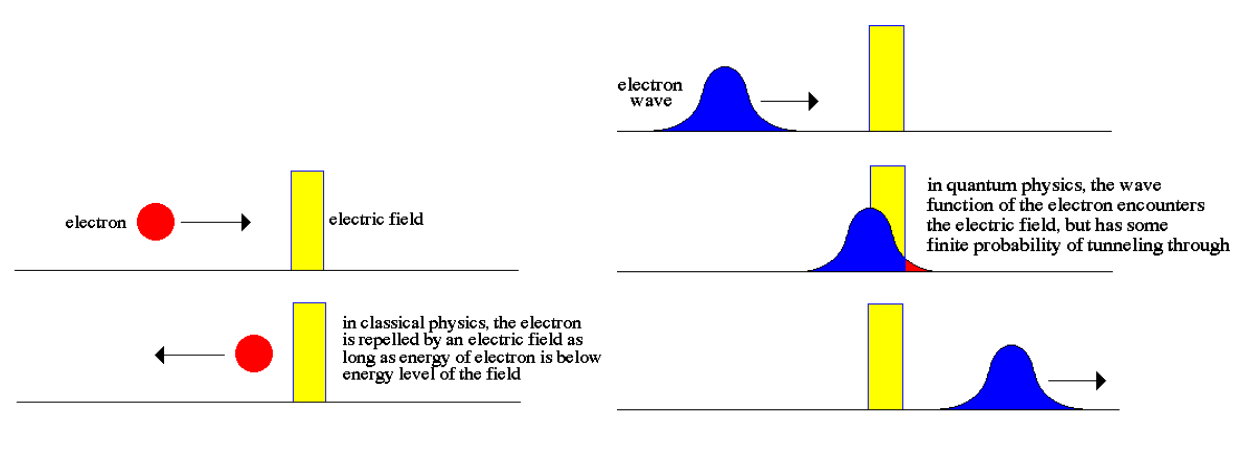
\includegraphics[width=\textwidth]{img/TunnelingAll.png}
        \caption{A visual representation of the quantum gates \autocite{imgtunnel}}
        \label{fig:quantum tunneling}
\end{figure}